%% Based on:

%%%%%%%%%%%%%%%%%%%%%%%%%%%%%%%%%%%%%%%%%
% a0poster Portrait Poster
% LaTeX Template
% Version 1.0 (22/06/13)
%
% The a0poster class was created by:
% Gerlinde Kettl and Matthias Weiser (tex@kettl.de)
% 
% This template has been downloaded from:
% https://www.latextemplates.com/template/a0poster-portrait-poster
%
% License:
% CC BY-NC-SA 3.0 (http://creativecommons.org/licenses/by-nc-sa/3.0/)
%
%%%%%%%%%%%%%%%%%%%%%%%%%%%%%%%%%%%%%%%%%


%----------------------------------------------------------------------------------------
%	PACKAGES AND OTHER DOCUMENT CONFIGURATIONS
%----------------------------------------------------------------------------------------

\documentclass[a0,portrait]{a0poster}

\usepackage{multicol} % This is so we can have multiple columns of text side-by-side
\columnsep=100pt % This is the amount of white space between the columns in the poster
\columnseprule=3pt % This is the thickness of the black line between the columns in the poster

\usepackage[svgnames]{xcolor} % Specify colors by their 'svgnames', for a full list of all colors available see here: http://www.latextemplates.com/svgnames-colors

%\usepackage{newtxtext} % Use the times font for text, newer flavor
\usepackage{helvet}
\renewcommand{\familydefault}{\sfdefault} % sans serif font

\usepackage{graphicx} % Required for including images
\graphicspath{{img/}} % Location of the graphics files
\usepackage{booktabs} % Top and bottom rules for table
\usepackage[font=small,labelfont=bf]{caption} % Required for specifying captions to tables and figures
\usepackage{amsfonts, amsmath, amsthm, amssymb} % For math fonts, symbols and environments
\usepackage{wrapfig} % Allows wrapping text around tables and figures

\usepackage{physics}
\usepackage[T1]{fontenc}
\usepackage[utf8]{inputenc}
\usepackage{setspace}

\usepackage{bbm}

\usepackage[top=2.8cm,right=2.8cm,bottom=2.8cm,left=2.6cm]{geometry}

%\usepackage{lipsum}

\usepackage[safeinputenc,doi=false,backend=biber]{biblatex}
\addbibresource{bib/main.bib}

% %% https://tex.stackexchange.com/a/366170
% \makeatletter
% \renewenvironment{abstract}{%
%   \begin{center}%
%     {\bfseries \large\abstractname\vspace{\z@}}
%   \end{center}%
%   \quotation
% }
% \makeatother

%----------------------------------------------------------------------------------------
% FROM tex/lib.tex
%----------------------------------------------------------------------------------------
% TODO: DRY
\newcommand{\term}[1]{\emph{#1}}
\newcommand{\idop}{\mathbbm{1}}           % Identity operator
\newcommand{\hilb}[1]{\mathcal{#1}}       % Hilbert space
\newcommand{\setof}[1]{\left\{#1\right\}}
\newcommand{\ox}{\otimes}
%
%% Allows better formatting than \underset
%% https://tex.stackexchange.com/a/130553
\DeclareMathOperator*{\repr}{\equiv}      % represented in a basis, or "has components..."
%
\renewcommand{\op}{\hat}                  % overwriting physics \op = \ketbra
\newcommand{\eqbydef}{\coloneqq}
%\newcommand{\eqbydef}{\triangleq}
\newcommand{\superop}{\mathcal}
%
\newcommand{\smallback}{\hspace{-0.115em}}
\newcommand{\largeback}{\hspace{-0.365em}}
%
\newcommand{\dket}[1]{\left.\left| #1 \right\rangle\smallback\right\rangle}
\newcommand{\Dket}[1]{\left.\left| #1 \right\rangle\largeback\right\rangle}
% and similar...
\newcommand{\dbra}[1]{\left\langle\smallback\left\langle #1 \right|\right.}
\newcommand{\dbraket}[2]{\left\langle\smallback\left\langle #1 \middle| #2 \right\rangle\right.}
\newcommand{\bradket}[2]{\left.\left\langle #1 \middle| #2 \right\rangle\smallback\right\rangle}
\newcommand{\dbradket}[2]{\left\langle\smallback\left\langle #1 \middle| #2 \right\rangle\smallback\right\rangle}
\newcommand{\dketdbra}[2]{\left| #1 \left\rangle\smallback\left\rangle \smallback \right\langle\smallback\right\langle #2 \right|}


%\renewcommand{\abstractname}{\large Abstract} % abstract hacks

\begin{document}
%----------------------------------------------------------------------------------------
%	POSTER HEADER 
%----------------------------------------------------------------------------------------
\begin{minipage}[c]{0.70\linewidth}%
%\vspace{1cm}
\veryHuge \color{NavyBlue} \textbf{Quantum Time: Page-Wootters and Detector\\[0.5cm] Models} \color{Black}\\[0.5cm] % Title
%\Huge\textit{Overcoming Pauli's Objection: Relational Time and \\Applications}\\[2cm] % Subtitle
\\[0.7cm]
\LARGE \textbf{Guido De Rosa, Andreas Ruschhaupt}\\[0.5cm] % Author(s)
\huge University College Cork, Department of Physics\\[0.4cm] % University/organization
\large%
\texttt{gderosa@umail.ucc.ie}
\end{minipage}%
%
\begin{minipage}[t]{0.25\linewidth}
\hspace{3cm}
\includegraphics[width=16cm]{ucc_logo.pdf}\\  %% vector, from original SVG
\end{minipage}

\vspace{2cm} % A bit of extra whitespace between the header and poster content

%----------------------------------------------------------------------------------------

\begin{multicols}{2} % This is how many columns your poster will be broken into, a portrait poster is generally split into 2 columns

%----------------------------------------------------------------------------------------
%	ABSTRACT
%----------------------------------------------------------------------------------------

\color{Navy} % Navy color for the abstract

\section*{\large Abstract}
%\noindent % abstract hacks
Here we compare the Page and Wootters (PaW) model of quantized time
(see \cite{PageWootters, Lloyd:Time},
or \cite{Moreva:illustration, Moreva_position} for experimental realizations)
with detection models based on absorption and loss of normalization
by a complex potential \cite{RuschhauptAbsorption}. We show that the prediction
of the Page--Wooters mechanism and of such detector model are compatible both in terms
of state evolution and time-of-arrival distribution. We do this by both ``plugging-in``
the imaginary absorption term (for detectors that strongly alter the system dynamics)
\emph{and} considering a weaker absorption regime, where the PaW model makes
the imaginary term in the Hamiltonian unnecessary. We emphasize how the probability
of detection in time is a \emph{conditional}
probability, in the Bayesian \cite{Maccone:QMOT} sense.


%\end{abstract}

\setlength{\parindent}{1.5em} % Default is 15pt.

%\color{SaddleBrown} % SaddleBrown color for the introduction

\large

\color{DarkSlateGray} % DarkSlateGray color for the rest of the content

\section*{Detector model: Complex potential of minimal uncertainty \cite{RuschhauptAbsorption}}

For a two-level system, if we consider:
\[
  \mathbf{K} = \hat{H} - i\hat{D} =
    \left[\begin{matrix}0 & 1\\1 & 0\end{matrix}\right] -
    \frac{i}{2} \left[\begin{matrix}0 & 0\\0 & \gamma \end{matrix}\right]
    \,\text{,}
\]
with an initial state of $\left[\begin{matrix}1\\0\end{matrix}\right]$,
minimal time-energy uncertainty is found with $\gamma = 2\sqrt{2}$.

Time-of-arrival distribution:
\begin{center}\vspace{1cm}
  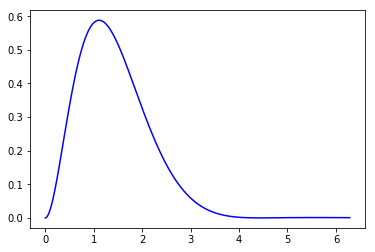
\includegraphics[width=0.4\linewidth]{2ldetect/toa-cont.png}
  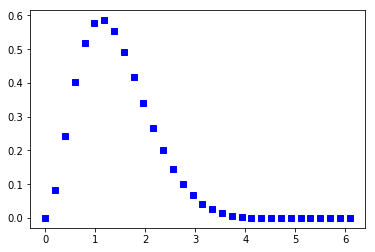
\includegraphics[width=0.4\linewidth]{2ldetect/toa-pw.png}
  \captionof{figure}{
    \color{Green}
    %Comparison of discrete P-W model prediction (points) with the ordinary QM Schr\"odinger solution (continuous line)
    %for eigensolutions of $\hat{\mathbb{J}}$ labeled as $\epsilon_{40}$ and $\epsilon_{41}$. Complex values.
  }
\end{center}\vspace{1cm}

\subsection*{Non-zero eigenvalues}

Up to an irrelevant global
phase, the physical vectors $\dket{\Psi}$ can be identified also by
imposing the constraint
\[
  \hat{\mathbb{J}}\dket{\Psi} = \epsilon \dket{\Psi}
\]
with real $\epsilon$. The corresponding evolution in $\hilb{H}_S$ will then need
a rigid energy shift of its spectrum by replacing $\ket{\psi(t)}_S$
with $e^{-i \epsilon t / \hbar} \ket{\psi(t)}_S$

\section*{Example: One qubit ``universe'' and a $N=32$-level clock}

The clock is built as having a time operator which is diagonal in the
chosen computational basis:
\[
  \hat{T} \repr \frac{2\pi}{N}
  \begin{pmatrix}
    0           &       &       &       \\
                &1      &       &       \\
                &       &\ddots &       \\
                &       &       &N-1
  \end{pmatrix} \,\text{.}
\]
With this choice, the clock spans the characteristic period of $\Delta T = 2\pi$.

The system is modeled by a 2-level Hamiltonian
\[
  \hat{H}_S \repr
  i \hbar \omega
  \begin{pmatrix}
    0   & 1   \\
    -1  & 0
  \end{pmatrix}
  \, \text{.}
\]

The frequency operator in $\hilb{H}_T$, as the canonically conjugate operator
of $\hat{T}$ in a finite-dimensional Hilbert space, is derived via
\emph{discrete Fourier transformation} \cite{FiniteHilb} (with $F_N$ unitary):
\[
  \hat{\Omega} = \frac{N}{2\pi} F^{}_{N} \hat{T} F^{\dagger}_{N} \, \text{.}
\]

We therefore need to find the eigenvectors of $\hat{\mathbb{J}}$ as in \eqref{eq:pwHamiltonian}
(a $2N \times 2N$ matrix obtained as a Kronecker product). Such eigensolutions
will encode the whole (periodic) evolution of the qubit (in $\hilb{H}_S$), but do
not ``evolve'' themselves (as there's no external ``time'' outside $\hilb{H}_T \ox \hilb{H}_S$).

In our example, we take $N = 32$ and resolve numerically.
With the chosen $\hat{H}_S$,
of some interest are solutions that show
Rabi oscillation / Larmor precession,
i.e. solutions that do not correspond to eigenstates of
the ``ordinary'' Hamiltonian $\hat{H}_S$ of the qubit.

We pick $\dket{\Phi_{40}}$ and $\dket{\Phi_{41}}$ corresponding to eigenvalues
$\epsilon_{40} = 12$ and $\epsilon_{41} = 11$.

The first two components of each eigenvector in the computational basis
are interpreted as the components of the qubit in $\hilb{H}_S$ at $t=0$. The components
$2k$\nobreakdash-th and $2k+1$\nobreakdash-th
as the components of the qubit at $k$-th discrete temporal step ($t = k \frac{2\pi}{N}$).
Comparison with ordinary quantum mechanics solution (Schr\"odinger equation) as shown in picture.

\begin{center}\vspace{1cm}
  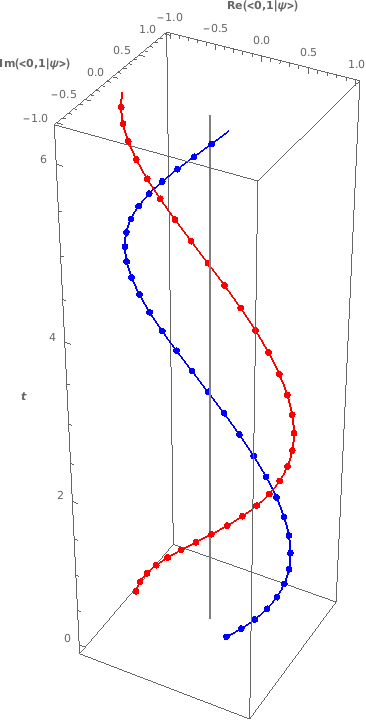
\includegraphics[width=0.3\linewidth]{PWfit32.png}
  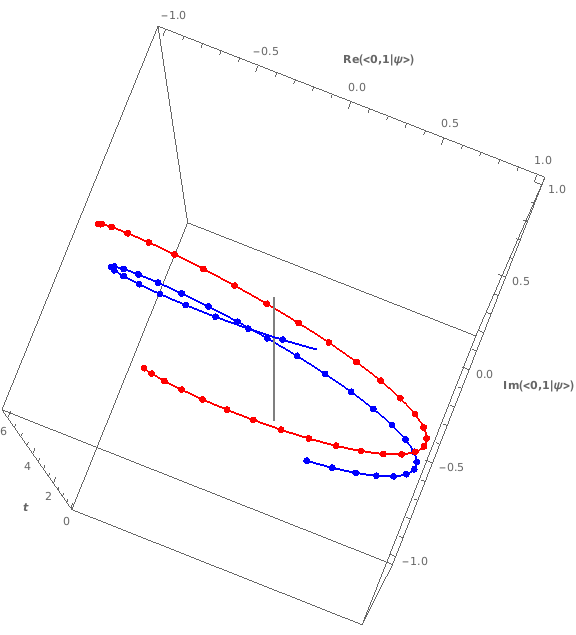
\includegraphics[width=0.4\linewidth]{PWfit32top.png}
  \captionof{figure}{
    \color{Green}
    Comparison of discrete P-W model prediction (points) with the ordinary QM Schr\"odinger solution (continuous line)
    for eigensolutions of $\hat{\mathbb{J}}$ labeled as $\epsilon_{40}$ and $\epsilon_{41}$. Complex values.
  }
\end{center}\vspace{1cm}

%----------------------------------------------------------------------------------------
%	CONCLUSIONS
%----------------------------------------------------------------------------------------

\color{SaddleBrown} % SaddleBrown color for the conclusions to make them stand out


% \section*{Conclusions and Outlook}

% \begin{itemize}
% \item Pellentesque eget orci eros. Fusce ultricies, tellus et pellentesque fringilla, ante massa luctus libero, quis tristique purus urna nec nibh. Phasellus fermentum rutrum elementum. Nam quis justo lectus.
% \item Vestibulum sem ante, hendrerit a gravida ac, blandit quis magna.
% \item Donec sem metus, facilisis at condimentum eget, vehicula ut massa. Morbi consequat, diam sed convallis tincidunt, arcu nunc.
% \item Nunc at convallis urna. isus ante. Pellentesque condimentum dui. Etiam sagittis purus non tellus tempor volutpat. Donec et dui non massa tristique adipiscing.
% \end{itemize}

\color{DarkSlateGray} % Set the color back to DarkSlateGray for the rest of the content

\normalsize

 %----------------------------------------------------------------------------------------
%	REFERENCES
%----------------------------------------------------------------------------------------

%\bibliographystyle{plain}
%\bibliography{bib/main}

%biblatex
\printbibliography

%----------------------------------------------------------------------------------------
%	ACKNOWLEDGEMENTS
%----------------------------------------------------------------------------------------

% \section*{Acknowledgements}

% Etiam fermentum, arcu ut gravida fringilla, dolor arcu laoreet justo, ut imperdiet urna arcu a arcu. Donec nec ante a dui tempus consectetur. Cras nisi turpis, dapibus sit amet mattis sed, laoreet.

%----------------------------------------------------------------------------------------

\end{multicols}
\end{document}
